\chapter{Determinant, Levi-Civita, Cross Products}
\label{ch:determinant}

This chapter is outside the flow of the course, but it formally introduces the determinant, which we invoke as a tool when solving for eigenvalues. We introduced the determinant for $2\times 2$ matrices in Section~\ref{sec:determinants:easy}. The rules to generalize this picture to higher-dimensional matrices become rather cumbersome and do not contribute any intuition for what the determinant \emph{means}. Rather than going over the iterative rules for calculating $N\times N$ determinants, we provide a concise definition and build a physical intuition for the determinant as an object used to calculate volumes.\sidenote{In this chapter there is a conspicuous absence of the metric. Without a machine to define distance, how does one measure volume? The answer is that volumes are defined relative to the volume of formed by using all of the basis vectors to bound a surface (a parallelpiped).} 


\section{2D Determinant is an Area}
\label{sec:determinants:2D}

We return to the question of making sense of the \textbf{determinant}\index{determinant} of a matrix. We reminded ourselves of the determinant of a $2\times 2$ matrix in Section~\ref{sec:determinants:easy}. The result was
\begin{align}
    \det M = M\aij{1}{1}M\aij{2}{2} - M\aij{1}{2} M\aij{2}{1} \ .
    \label{eq:detM:2:expand}
\end{align}
You should be comfortable taking the determinant of a $2\times 2$ matrix using the above expression. For slightly larger matrices, there are recursive expressions that one may derive---but these are such a pain to use that in any practical modern application you would use a computer algebra system. So rather than spending time on that recursion relation, let us actually learn what a determinant \emph{is} in a way that can be written non-recursively for a matrix of any dimension.

So what is the determinant?\sidenote{The definition below is standard, but the proof in two dimensions and the extension to higher dimensions is not something I have seen in other textbooks.}
\begin{bigidea}[The determinant is an area]\label{idea:det:area}
The determinant of a $2\times 2$ matrix $M$ is the area of a parallelogram formed using the two vectors $M\ket{e_1}$ and $M\ket{e_2}$. 
\end{bigidea}
This area is relative to the area of the square formed by $\ket{e_1}$ and $\ket{e_2}$. If $\text{Area}(\vec{v}, \vec{w})$ is the area of the parallelogram formed by $\ket{v}$ and $\ket{w}$---forgive the mixed notation for the vectors---then
\begin{align}
    \text{Area}(M\bas{e}_1, M\bas{e}_2) = 
    \det M \; \text{Area}(\bas{e}_1, \bas{e}_2) 
    \ .
\end{align}
This definition \emph{had} to be so because we are not actually using the metric anywhere, so we have not defined distance let alone area. 

The general definition of a determinant in $N$ dimensions is that of an $N$-volume. In order to see that, we start by understanding why \bigidearef{}~\ref{idea:det:area} should be true. We assume that we have the standard basis, $\ket{e_1}$ and $\ket{e_2}$ and that they define a unit area. Figure~\ref{fig:det:the:vectors} shows the image (what they transform into) of these basis vectors under the action of the matrix $M$.
\begin{marginfigure}%[th]
    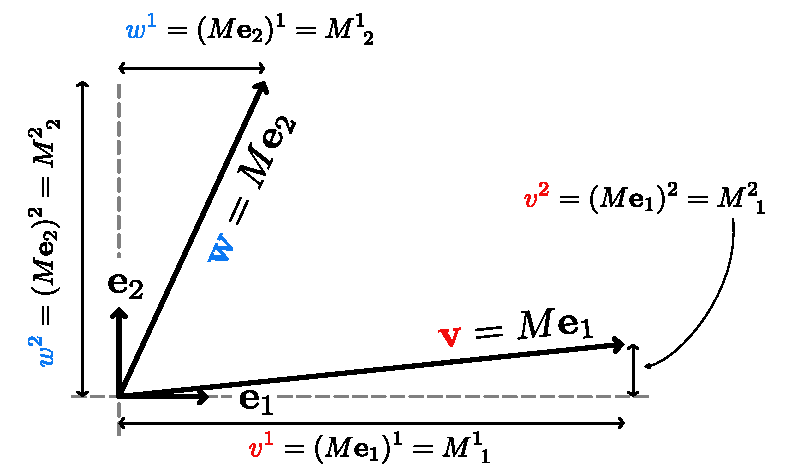
\includegraphics[width=\textwidth]{figures/det TheVectors.pdf}
    \captionsetup{font={scriptsize,sf}}
    \caption{Sketch of the standard basis $\ket{e_{1,2}}$ and their transformation under the matrix $M$.}
    \label{fig:det:the:vectors}
\end{marginfigure}
We write $\ket{v} = M\ket{e_1}$ and $\ket{w} = M\ket{e_2}$. Observe that the components of these vectors are simply the components of the matrix $M$:\sidenote{Appreciate that the heights of the indices in $\la e^i \mid M \mid e_j \ra$ helps keep track of whether this evaluates to $M\aij{i}{j}$ or $M\aij{j}{i}$.} Having mapped this out, our claim is that the determinant of $M$ is the area shown in Figure~\ref{fig:det:area}.
\begin{align}
    v^1 &= \la e^1 \mid v\ra = \la e^1 \mid M \mid e_1 \ra  = M\aij{1}{1}
    \label{eq:det:v1:inner:prod}
    \\
    v^2 &= \la e^2 \mid v\ra = \la e^2 \mid M \mid e_1 \ra = M\aij{2}{1}
    \\ 
    w^1 &= \la e^1 \mid w\ra = \la e^1 \mid M \mid e_2 \ra  = M\aij{1}{2}
    \\
    w^2 &= \la e^2 \mid w\ra = \la e^2 \mid M \mid e_2 \ra = M\aij{2}{2}
    \label{eq:det:w2:inner:prod}
    \ .
\end{align}
Here we are simply using the identification that $\la e^i |$ is a machine that takes in a vector and outputs its $i^\text{th}$ component, as we showed in \eqref{eq:dual:basis:returns:ith:component:ket}.
\begin{marginfigure}%[th]
    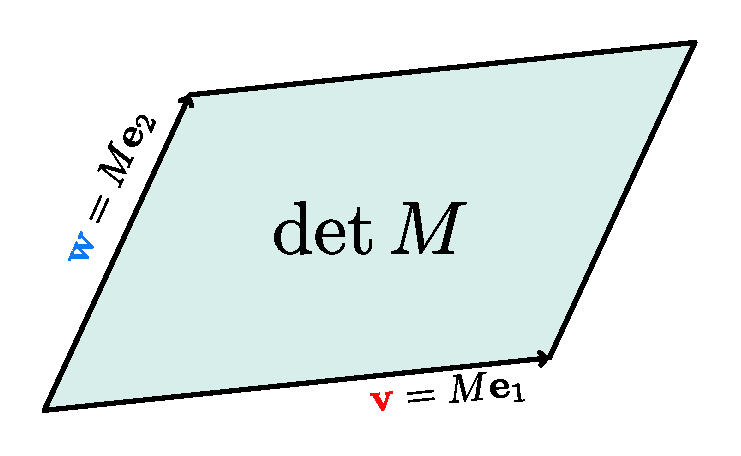
\includegraphics[width=\textwidth]{figures/det ParallelogramDet.pdf}
    \captionsetup{font={scriptsize,sf}}
    \caption{The area of this parallelogram formed out of $\ket{v} = M\ket{e_1}$ and $\ket{w}= M\ket{e_2}$ is the determinant of $M$.}
    \label{fig:det:area}
\end{marginfigure}
\begin{exercise}
Following the analysis argue that in any dimension, the \emph{columns} of a matrix $M\aij{i}{j}$ correspond to the vectors obtained by acting with $M$ on the basis vectors. That is to say: $M\aij{i}{j}$ is the $i^\textnormal{th}$ component of $M\ket{e_j}$. 

\textsc{Comment}: this is something I always get mixed up: are they the rows or the columns that matter? The heights of the indices are helpful reminder: the basis vectors are labeled by a lower index and vector components are labeled by an upper index.
\end{exercise}

It helps to peek at the proposed answer. \eqref{eq:detM:2:expand} tells us that the determinant is $M\aij{1}{1}M\aij{2}{2} - M\aij{1}{2} M\aij{2}{1}$. We now understand that each of the components maps onto one of the components of $\vec{v}=M\vec{e_1}$ or $\vec{w}=M\vec{e_2}$,
\begin{align}
    \det M = M\aij{1}{1}M\aij{2}{2} - M\aij{1}{2} M\aij{2}{1} 
    = v^1 w^2 - w^1 v^2 
    \ .
\end{align}
Lets proceed step by step. 

\paragraph{Difference of two boxes} We may interpret each of the two terms as the area of a rectangle on the plane, see Figure~\ref{fig:det:vis:boxes}. Our task then reduces to explaining why the difference of two rectangles should match the area of the parallelogram formed by $\vec{v}$ and $\vec{w}$. The first term, $v^1w^2$, is the area given by the yellow box in Figure~\ref{fig:det:vis:boxes}. Similarly, the second term, $v^2w^1$ is the area given by the blue box.
\begin{marginfigure}%[th]
    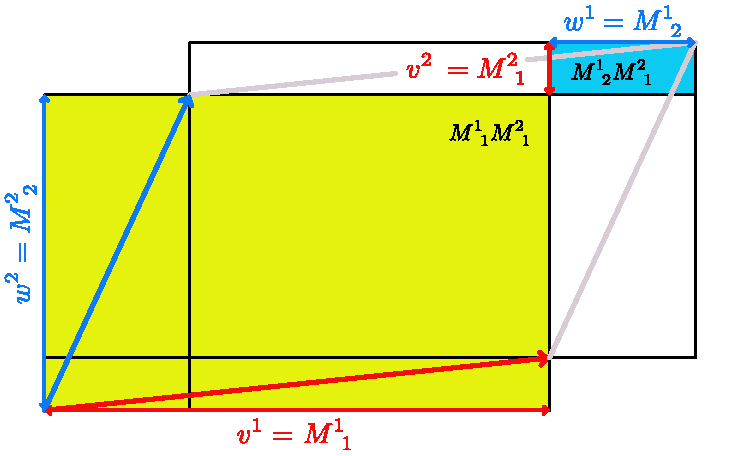
\includegraphics[width=\textwidth]{figures/det TwoPiecesofDet.pdf}
    \captionsetup{font={scriptsize,sf}}
    \caption{The expression \eqref{eq:detM:2:expand} for $\det M$ is the difference between the yellow and blue boxes.}
        \label{fig:det:vis:boxes}
\end{marginfigure}

\paragraph{Covering the parallelogram} Compare the yellow box in Figure~\ref{fig:det:vis:boxes} to the parallelogram in Figure~\ref{fig:det:area}. We see that the yellow box of area $v^1w^2$ overlaps with the parallelogram except in two triangular areas, highlighted as the green and pink triangles on the bottom-left of Figure~\ref{fig:det:vis:triangles}. That figure shows that that we can rearrange the green and pink triangles to the upper-right of the box to fully cover the area of the parallelogram. 
\begin{marginfigure}%[th]
    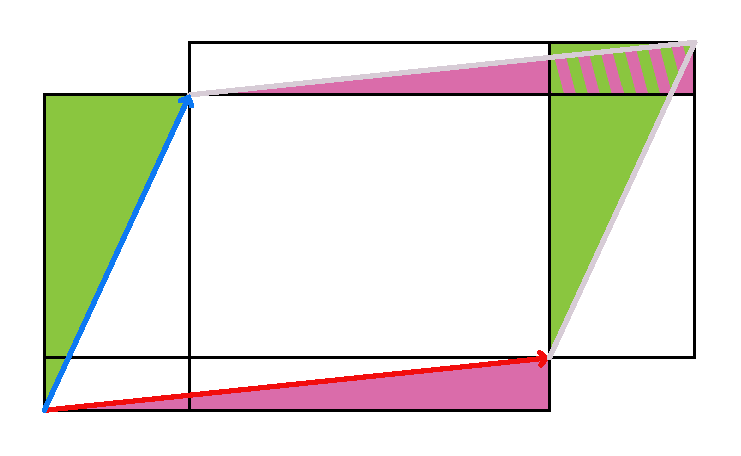
\includegraphics[width=\textwidth]{figures/det TwoPiecesofDetall.pdf}
    \captionsetup{font={scriptsize,sf}}
    \caption{The expression \eqref{eq:detM:2:expand} for $\det M$ is the difference between the yellow and blue boxes.}
    \label{fig:det:vis:triangles}
\end{marginfigure}

\paragraph{Overcounting} In Figure~\ref{fig:det:vis:triangles}, after moving the green and pink triangles to the top right, we see that we are \emph{overcounting} the area of the parallelogram. The cross-colored green/pink region are regions in the parallelogram that have been double counted. On top of this, the blue regions in Figure~\ref{fig:det:vis:extra} are counted in the yellow rectangle of Figure~\ref{fig:det:vis:boxes}  but are not part of the area of the parallelogram. If we rearrange them to the upper right of the diagram, we see that they combine with the double-counted region to recreate the $v^2w^1$ area of the blue box in Figure~\ref{fig:det:vis:boxes}. 

\bigskip
We thus confirm \bigidearef{}~\ref{idea:det:area} where we stated that our formula \eqref{eq:detM:2:expand} for the determinant of a $2\times 2$ matrix $M$ represents the area of the parallelogram formed out of $\ket{v}=M\ket{e_1}$ and $\ket{w} = M\ket{e_2}$.

\begin{marginfigure}%[th]
    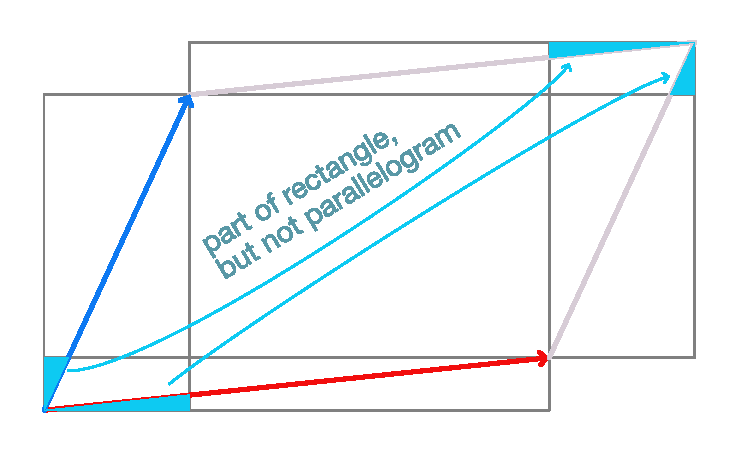
\includegraphics[width=\textwidth]{figures/det TwoPiecesofDetExtraTeal.pdf}
    \captionsetup{font={scriptsize,sf}}
    \caption{The blue triangles in the lower left are counted in the area $v^1w^2$ but, upon rearranging the green and pink triangles in Figure~\ref{fig:det:vis:triangles}, represent an area that is \emph{not} part of the parallelogram. Combining these two triangles with the cross-colored region of Figure~\ref{fig:det:vis:triangles} recovers the blue box of area $v^2w^1$ in Figure~\ref{fig:det:vis:boxes}.}
    \label{fig:det:vis:extra}
\end{marginfigure}


Our proposal for the general definition of the determinant in any dimension is as follows:
\begin{bigidea}[The determinant is a volume]\label{idea:det:volume}
The determinant of a $N\times N$ matrix $M$ is the (hyper-)volume of a parallelpiped formed out of the vectors $M\ket{e_1}$, $\cdots$, $M\ket{e_N}$. Here `parallelpiped' is the $N$-dimensional version of a two-dimensional parallelogram.
\end{bigidea}
In order to go from the $2\times 2$ area that we have shown here to higher dimensions, we introduce another big idea: the Levi-Civita\sidenote{This is named after Tullio Levi-Civita rather than being a compound of two different names. As such, typographically we use a dash to signify a compound last name. This is in contrast to ideas that are named after pairs of people, such as the Randall--Sundrum model. In the latter case, we typographically use something called an \emph{en-dash} (it is the width of the letter `n') to separate the two names.} symbol.


\section{Levi-Civita Symbol}

We motivate the Levi-Civita symbol by writing the expression for the determinant of a $2\times 2$ matrix \eqref{eq:detM:2:expand} in terms of the two-dimensional Levi-Civita:
\begin{align}
    \det M = \epsilon_{ij}M\aij{i}{1} M\aij{j}{2} \ .
    \label{eq:detM:2:eps:ij}
\end{align}
Even without defining $\epsilon_{ij}$, you can guess the components simply by comparing the two expressions for the determinant:
\begin{align}
    \begin{pmatrix}
        \epsilon_{11} & \epsilon_{12} \\
        \epsilon_{21} & \epsilon_{22} 
    \end{pmatrix}
    =
    \begin{pmatrix}
        \pp 0 & 1 \\
        -1 & 0
    \end{pmatrix} \ .
\end{align}
% 
\begin{exercise}
Explicitly write out the sum in \eqref{eq:detM:2:eps:ij} to show that it equals the right-hand side of \eqref{eq:detM:2:expand}.
\end{exercise}
% 
The object $\epsilon_{ij}$ is called the two-dimensional \textbf{Levi-Civita} symbol\index{Levi-Civita symbol}.\sidenote{We deliberately call this object a \emph{symbol} instead of a \emph{tensor}. In the context of this course, the two are interchangeable---but the distinction between the two is a big deal in field theory.} A mathematical definition is:
\begin{align}
    \epsilon_{ij} = 
    \begin{cases}
    \pp 1 &\text{if }\{i,j\}\text{ is an even permutation of }\{1,2\}\\
    -1 &\text{if }\{i,j\}\text{ is an odd permutation of }\{1,2\}\\
    \pp 0 &\text{otherwise}
    \end{cases}
    \ .
\end{align}
By \emph{permutation} we mean some rearrangement of the list. Whether a permutation is even or odd is based on whether you can reach that permutation by doing an even or an odd number of component swaps.

\begin{example}
$\{1,3,2,4\}$ is an even permutation of $\{1,2,3,4\}$ but $\{2,1,3,4\}$ is an odd permutation.
\end{example}


\begin{wide}
In a $d$-dimensional vector space one may use the Levi-Civita symbol with $d$-indices, defined as
\begin{align}
    \epsilon_{i_1\cdots i_d} \defeq 
    \begin{cases}
    \pp 1 &\text{if }\{i_1,\cdots, 1_d\}\text{ is an even permutation of }\{1,\cdots, d\}\\
    -1 &\text{if }\{i_1,\cdots, 1_d\}\text{ is an odd permutation of }\ \{1,\cdots, d\}\\
    \pp 0 &\text{otherwise}
    \end{cases} \ .
    \label{eq:Levi:Civita:symbol:definition:d:dim}
\end{align}
\end{wide}
We say that the Levi-Civita symbol is \emph{totally antisymmetric}\sidenote{\emph{Totally antisymmetric} is not valleyspeak.\footnotemark We mean that the interchange of \emph{any} two indices introduces a minus sign.} in its indices.\footnotetext{\cite{suh2011social} }

\begin{example}
In three dimensions
\begin{align}
\epsilon_{123} &=
\epsilon_{312} = 
\epsilon_{231} = \pp 1
\\
\epsilon_{213} &= 
\epsilon_{321} = 
\epsilon_{132} = -1 
\end{align}
with all other values zero.
\end{example}

There is also an upper-index version of the Levi-Civita symbol. By convention we choose it to have the same components as the lower-indexed version:
\begin{align}
    \epsilon^{i_1\cdots i_d}
    \defeq
    \epsilon_{i_1\cdots i_d} \ .
    \label{eq:def:levi:civita:d:dim:upper}
\end{align}
Be clear that this is a \emph{choice}. We could have just as validly defined the two components to differ by an overall sign.

\section{Where did Levi-Civita come from?} 

The Levi-Civita symbol is totally antisymmetric\index{antisymmetric} under permutations of its indices. We motivate the significance of permutation symmetry for tensors with multiple upper or lower indices in Section~\ref{sec:permutation:symmerty}. Tensors in two dimensions with two lower indices may be written in terms of a symmetric and antisymmetric part $T_{ij}= S_{ij} + A_{ij}$. One may write the antisymmetric part in terms of the two-component Levi-Civita symbol,
\begin{align}
    A_{ij} = \epsilon_{ij} \frac{1}{2} \left(A_{12}-A_{21}\right)
    =\epsilon_{ij} A_{12}
     \ .
    \label{eq:antisymmetric:wrt:levi:civita}
\end{align}
One may read this as the product of a factor $\epsilon_{ij}$ that enforces the antisymmetry of the indices and a factor that represents the average over the totally antisymmetric part of the tensor $A$, which by definition is the antisymmetric part of $T$.
\begin{exercise}
Generalize the above expression for the antisymmetric part $A$ of a tensor in $d$-dimensions with $d$ indices in terms of the $d$-index Levi-Civita tensor.
\end{exercise}
One of the neat things about separating out the totally symmetric and totally antisymmetric parts of a tensor is that those pieces tend to transform among themselves. Isometries will take totally symmetric tensors to totally symmetric tensors and totally antisymmetric tensors to totally antisymmetric tensors. This observation is useful when decomposing representations of groups.

\paragraph{Where did this really come from?}
% 
The Levi-Civita tensor is also the index-based manifestation of an idea called \textbf{Hodge duality}\index{Hodge duality} in differential geometry.\sidenote{If only I could use this sentence when kids used to ask me ``where are you \emph{really} from?'' when I was growing up.} While this is outside the scope of our course, this duality is related to interchange of electric and magnetic fields in the absence of sources in Maxwell's equations. From a tensorial perspective, the manifestation of the duality is that the Levi-Civita tensor in $d$ dimensions can contract with a tensor $T^{i_1\cdots i_p}$ with $p$ upper indices to return a `dual' object with $(d-p)$ totally antisymmetric indices
\begin{align}
   \tilde T_{j_{(d-p)}\cdots j_{d}} 
   = 
   \epsilon_{j_1 \cdots j_d}  T^{j_1 \cdots j_p} \ .
   \label{eq:Hodge:duality:epsilon}
\end{align}
This idea is just below the surface of a chunk of electrodynamics
~\autocite{Fumeron:2020bjj}. Another closely related invitation to this topic is called geometric algebra, \autocite{Doran:2007tqa}.

\begin{exercise}
Show that the Hodge dual $\epsilon^{\mu\nu\alpha\beta}F_{\alpha\beta}$ of the electromagnetic field strength tensor $F_{\mu\nu}$ in \eqref{eq:fmunu:lower} swaps swaps electric and magnetic fields relative to $F^{\mu\nu}$. This  \emph{electromagnetic duality} is a discrete symmetry of Maxwell's equations in the absence of sources. 
\end{exercise}

\section{Antisymmetry Gymnastics}
\label{sec:antisymmetric:dynamics}

\paragraph{(Anti-)Symmetrizing Over Indices}
The Levi-Civita symbol is a powerful tool for working with antisymmetric tensors. First, we introduce a handy notation for indicating the symmetric and antisymmetric parts of a tensor. We define any indices of the same height that are enclosed in round brackets as being symmetrized. For example, over three indices: 
\begin{align}
    T^{(ijk)} = \frac{1}{3!}\left(T^{ijk} + T^{jik} + T^{kji}
                      + T^{ikj} + T^{kij} + T^{jki}\right) \ .
\end{align}
The factor of $1/3!$ is a convention to account for the fact that we are \emph{averaging} over the three indices. Square brackets indicate \emph{anti}-symmetrization over the enclosed indices:
\begin{align}
    T^{(ijk)} = \frac{1}{3!}\left(T^{ijk} - T^{jik} + T^{kji}
                      + T^{ikj} - T^{kij} - T^{jki}\right) \ .
\end{align}
The generalization to $n$ enclosed indices is understood to be
\begin{align}
    T^{(i_1\cdots i_n)} &= 
    \frac{1}{n!}\sum_{\sigma} \phantom{(\sgn{\sigma})} T^{\sigma_1\cdots\sigma_n}
    \\
    T^{[i_1\cdots i_n]} &= 
    \frac{1}{n!}\sum_{\sigma} (\sgn{\sigma}) T^{\sigma_1\cdots\sigma_n} \ ,
\end{align}
where $\sigma$ is a permutation of the $n$ indices and $\sgn(\sigma)$ is $\pm 1$ depending on whether the permutation is even or odd. 

\paragraph{Levi-Civita and Antisymmetrized Indices}
The Levi-Civita tensor lets us write the antisymmetric piece of a tensor by factoring out the indices. \eqref{eq:antisymmetric:wrt:levi:civita} demonstrates this in two dimensions. For our purposes, let us consider antisymmetrization of $d$ indices in a $d$-dimensional vector space
\begin{align}
    T_{[i_1\cdots i_d]} = 
    \epsilon_{i_1\cdots i_d}
    T_{1\cdots d} \ .
    \label{eq:totally:antisymmetric:propto:epsilon}
\end{align}
\begin{example}\label{eg:pull:out:epsilon}
Suppose you have a totally antisymmetric tensor $A^{[i\cdots k]}$. This object has $k$ indices, but they have been fully antisymmetrized. Once you know any one non-zero component, you know all of the components---the tensor contains one number's worth of information. \eqref{eq:totally:antisymmetric:propto:epsilon} defines that one number as the element $A^{1\cdots d}$. We may reconstruct $A^{[i\cdots k]}$ by using $\epsilon^{i_1\cdots i_d}$ to insert the index-dependence:
\begin{align}
    A^{[i\cdots k]} = \epsilon^{i\cdots k} \, A^{1\cdots d}
\end{align}
\end{example}

\paragraph{Antisymmetric Products of Matrices}
We often find ourselves antisymmetrizing over indices multiple matrices. For example,
\begin{align}
    M\aij{i}{[k}M\aij{j}{\ell]} &\defeq
    \frac{1}{2}
    \left(M\aij{i}{k}M\aij{j}{\ell} - M\aij{i}{\ell}M\aij{j}{k} \right) \ .
\end{align}
We can then use the fact that $M\aij{a}{b}M\aij{c}{d} = M\aij{c}{d} M\aij{a}{b}$ in order to convert the antisymmetrization of the lower matrix indices to the antisymmetrization of the upper indices:
\begin{align}
    M\aij{i}{[k}M\aij{j}{\ell]}
    = 
    M\aij{[i}{k}M\aij{j]}{\ell} \ .
    \label{eq:moving:antisymmetrization:up}
\end{align}
\begin{exercise}
Prove \eqref{eq:moving:antisymmetrization:up} and argue that it generalizes to
\begin{align}
   M\aij{i}{[\ell} M\aij{j}{m} \cdots M\aij{k}{n]} 
   =
   M\aij{[i}{\ell} M\aij{j}{m} \cdots M\aij{k]}{n} \ .
   \label{eq:antisymmetrize:goes:up}
\end{align}
\end{exercise}
\begin{exercise}
Show that \eqref{eq:detM:2:eps:ij} is equivalent to 
\begin{align}
    \det M = \epsilon^{ij} M\aij{1}{i}M\aij{2}{j}
\end{align}

\end{exercise}


\begin{exercise}
Show that the arguments for antisymmetrized indices also hold for symmetrized indices.
\end{exercise}

\paragraph{Pulling out the antisymmetric part}
Because $\epsilon_{ij}$ `annihilates' the symmetric part of $M\aij{i}{k}M\aij{j}{\ell}$, we have
\begin{align}
    \epsilon_{ij}
    M\aij{i}{k}M\aij{j}{\ell}
    &=
    \epsilon_{ij}
    M\aij{i}{[k}M\aij{j}{\ell]} \ .
    \label{eq:det:invariant:int:lemma:eps:M:anti}
\end{align}

\paragraph{A word of caution}
Please be \emph{very} clear that \eqref{eq:antisymmetrize:goes:up} \emph{depends} on the fact that $M\aij{a}{b}M\aij{c}{d} = M\aij{c}{d} M\aij{a}{b}$. The generalization \eqref{eq:antisymmetrize:goes:up} also depends on the fact that you have products of the \emph{same} matrix which imposes a symmetry between the indices.\sidenote{Please appreciate that this symmetry is simple to see because of our index notation, as we first suggested in Example~\ref{eg:moving:coefficients:around}.} If one were acting on a general tensor $T\aij{ab}{cd}$, then symmetrizing or antisymmetrizing the upper indices does \emph{not} imply anything about the lower indices. What was special about the tensor $W\aij{ab}{cd} \equiv M\aij{a}{b}M\aij{c}{d}$ is that its definition implies a key relationship:
\begin{align}
    W\aij{ab}{cd} = W\aij{ba}{dc} \ ,
\end{align}
which is ultimately what we used in the previous two exercises. It is \emph{not} true in general that $W\aij{(ab)}{cd} = W\aij{ab}{(cd)}$ or that $W\aij{[ab]}{cd} = W\aij{ab}{[cd]}$.


\section{Levi-Civita and the Determinant}
\label{sec:levi:civita:determinant}

The Levi-Civita symbol allows us to formalize the definition of the determinant as a volume of a parallelpiped in \bigidearef{}~\ref{idea:det:volume}:\sidenote{Some authors define $|M| = \det M$ to mean the determinant of a matrix $M$. We avoid this potentially confusing notation because there are other contexts---such as on spacetime---where one has to write the absolute value of the determinant.}
\begin{align}
    \det M \defeq \epsilon_{i_1 \cdots i_d} M\aij{i_1}{1}\cdots M\aij{i_d}{d} \ .
    \label{eq:levi:civita:determinant:definition}
\end{align}
\begin{exercise}
Use your antisymmetrization gymnastics to show that
\begin{align}
    \det M = \frac{1}{n!}
    \epsilon_{i_1 \cdots i_d}
    \epsilon^{j_1 \cdots j_d}
    M\aij{i_1}{j_1}\cdots M\aij{i_d}{j_d} \ .
    \label{eq:levi:civita:determinant:definition:totally:antisymmetrized}
\end{align}
\end{exercise}
This definition is a clear generalization of \eqref{eq:detM:2:eps:ij}. We now show that this definition allows us to iteratively generalize the geometric argument in Section~\ref{sec:determinants:2D} to successively higher dimensions. The result of that argument is that for a $2\times 2$ matrix $M$ the area of a parallelogram formed out of $\ket{v}=M\ket{e_1}$ and $\ket{w}=M\ket{e_2}$. 

\paragraph{Volume of a parallelpiped}
We extend that two-dimensional space with a third dimension. This means that $M$ is now a $3\times 3$ matrix. We \emph{choose coordinates} so that $\ket{e_1}$ and $\ket{e_2}$ are the same in the three-dimensional space as they were in the two-dimensional space. That is: we have simply augmented the space Section~\ref{sec:determinants:2D} with a third orthonormal basis direction, $\ket{e_3}$. We show this in Figure~\ref{fig:det:parallelpiped}. 
\begin{marginfigure}%[th]
    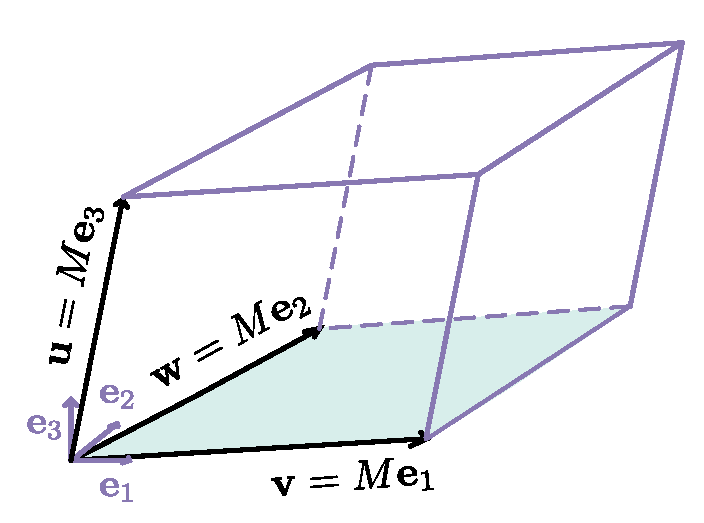
\includegraphics[width=\textwidth]{figures/det Parallelpiped.pdf}
    \captionsetup{font={scriptsize,sf}}
    \caption{Three dimensional extension of Fig.~\ref{fig:det:area}. In general the parallelogram is not aligned with the $\ket{e_{1,2}}$ basis. We define the basis $\ket{f_i}$ to be that where the $\ket{v}$ and $\ket{w}$ vectors live on the $\ket{f_{1,2}}$ plane.}
    \label{fig:det:parallelpiped}
\end{marginfigure}

The old $2\times 2$ matrix $M$ now occupies the upper-left corner of the new $3\times 3$ matrix $M$. In general, $M\ket{e_1}$  and $M\ket{e_2}$ are not in the same plane as $\ket{e_{1}}$ and $\ket{e_2}$. We may \emph{choose} a new basis $\ket{f_{1,2}}$ that lives on the same plane as $M\ket{e_{1,2}}$.  We then choose a third orthonormal basis vector, $\ket{e'_3}$. In this new basis, $\ket{v} = (v')^i\ket{f_i}$ and $\ket{w}=(w')^i\ket{f_i}$ are on the $\ket{f_{1,2}}$ plane. The area of the parallelogram on this plane formed by $\ket{v}$ and $\ket{w}$ is still
\begin{align}
    \text{Area of parallelogram} = \epsilon_{ij}(v')^i(w')^j \ .
\end{align}
There is a third vector $\ket{u} = M\ket{e_3} = (u')^i \ket{f_i}$ that we use to form the parallelpiped out of the parallelogram. 

Given that we are in three dimensions, the natural object is the Levi-Civita symbol with three indices, $\epsilon_{ijk}$. In the $\ket{f_{i}}$ basis, we may construct the following object:
\begin{align}
    \epsilon_{ijk}\;(v')^i(w')^j \ .
\end{align}
By construction, $(v')^i$ and $(w')^j$ are zero for $i,j=3$. However, $\epsilon_{ijk}$ above is \emph{only} non-zero when $\{i,j,k\}$ is a permutation of $\{1,2,3\}$. If This means that the only non-zero term in this sum over $i$ and $j$ is the case when $k=3$. This means:
\begin{align}
    \epsilon_{ijk}\;(v')^i(w')^j
    &=
    \begin{cases}
    0 &\text{if } k = 1,2\\
    \epsilon_{ab}(v')^a (v')^b &\text{if } k = 3
    \end{cases} \ ,
    \label{eq:det:eps:v:w}
\end{align}
where $a$ and $b$ only take values 1 or 2. The first two components vanish, and the third component is simply the area of the parallelogram formed out of $\ket{v}$ and $\ket{w}$. 

The dual vector $\epsilon_{ijk}\;(v')^i(w')^j$ takes in a vector and returns the product of the third component of that vector with the area of the parallelogram formed out of $\ket{v}$ and $\ket{w}$. The natural thing to do is to fee this dual vector our one remaining vector, $\ket{u}$. Because $\epsilon_{ijk}\;(v')^i(w')^j$ projects out the third component, it multiplies the area of the parallelogram by the `height' of the vector $\ket{u}$ relative to the plane of the parallelogram. This is simply the volume of the parallelpiped:
\begin{align}
    V = \epsilon_{ijk}\;(v')^i(w')^j(u')^k \ .
\end{align}
We now have a way of writing the volume of the parallelpiped formed out of the vectors $M{\ket{e_i}}$. This is precisely our definition of the determinant in \bigidearef{}~\ref{idea:det:volume}. The expression was derived in terms of the components in the $\ket{f_i}$ basis. However, you may intuit that the volume of the parallelpiped is basis independent. This is indeed true, with one small caveat.

The components (primed) in the $\ket{f_i}$ basis are related to the components (unprimed) in the $\ket{e_i}$ basis by a rotation, $(v')^i=R\aij{i}{j}v^i$, and similarly for $(w')^i$ and $(u')^i$. If we plug this into our expression for the volume of the parallelpiped,
\begin{align}
    V' = \epsilon_{ijk}\; 
    R\aij{i}{\ell}
    R\aij{j}{m}
    R\aij{k}{n}
    v^\ell w^m u^n \ .
\end{align}
Using some of our antisymmetry gymnastics, we see that antisymmetrizing in the $ijk$ indices also antisymmetrizes the $\ell m n$ indices so that
\begin{align}
    V' = \epsilon_{ijk}\; 
    R\aij{i}{1}
    R\aij{j}{2}
    R\aij{k}{3}\;
    \epsilon_{\ell m n}
    v^\ell w^m u^n 
    =
    (\det R)\; V
    \ .
\end{align}
On the right-hand side we identify $V=\epsilon_{\ell m n} v^\ell w^m u^n $, the volume one would measure in the original basis. We see that these are equivalent when $\det R = 1$. For ordinary rotations this is always the case.\sidenote{This is because rotations preserve the inner product and so preserve the length and relative angles of vectors. This, in turn, is related to \eqref{eq:det:v1:inner:prod}--\eqref{eq:det:w2:inner:prod} because the bras are defined with respect to the inner product \emph{a la} \eqref{eq:basis:dual:vectors:as:inner:prod}.} That means we can simply write the volume $V$ of the parallelpiped in terms of the components $M\aij{i}{j}$ in the original basis:
\begin{align}
    V = \epsilon_{ijk}
    M\aij{i}{1}
    M\aij{j}{2}
    M\aij{k}{3}
    = \det M \ ,
\end{align}
where we have used the same arguments as \eqref{eq:det:v1:inner:prod}--\eqref{eq:det:w2:inner:prod} to show that $M\aij{i}{j} = \la e^i \mid M e_j \ra $ . 

\begin{exercise}
Show by explicit component-wise calculation that the standard form of a $2\times 2$ rotation matrix satisfies $\det R = 1$. 
\end{exercise}

\paragraph{Generalization to higher dimensions}

The arguments above show how to use the Levi-Civita symbol to take the `volume' (area) formed by two vectors into the volume formed by three vectors. By identifying these vectors as the image of a matrix acting on the basis vectors, $M\ket{e_i}$, we were able to bootstrap a connection between the Levi-Civita definition of the determinant of a $3\times 3$ matrix \eqref{sec:levi:civita:determinant} and the geometric picture of a volume in \bigidearef{}~\ref{idea:det:volume}.

You may iterate this step by taking the volume of a three-dimensional parallelpiped and then imagining that this is embedded in some four-dimensional space. 
\begin{enumerate}
    \item The 3-parallelpiped are then one three-dimensional face of the four-dimensional 4-parallelipied.
    \item  By judicious choice of basis, $\ket{f_i}$, the dual vector component $\epsilon_{ijk\ell}(v')^i(w')^j(u')^k$ is only non-zero when $\ell=4$.
    \item  Acting on the fourth vector with this dual vector then gives the volume of the 4-paralellpiped.
    \item  We recognize that this number is invariant under rotations and so we may write it in the original basis. In that basis, the components of the four vectors are simply the columns of the matrix $M$ and so the expression for the 4-volume is the determinant of $M$.
\end{enumerate}


\paragraph{Unusual Isometries} The primary weakness of the arguments above is that we were quick to say that the determinant of an ordinary rotation is one. You can check this is true for the rotations that we have explored thus far in this course. However, it is not true for all isometries. 

\begin{exercise}\label{ex:orientation:2d}
Show that the matrix
\begin{align}
    \tilde R = 
    \begin{pmatrix}
        \tilde R\aij{1}{1} & \tilde R\aij{1}{2}\\
        \tilde R\aij{2}{1} & \tilde R\aij{2}{2}
    \end{pmatrix}
    =
    \begin{pmatrix}
     1 & 0 \\
     0 & -1   
    \end{pmatrix}
\end{align}
is an isometry. Show that
\begin{align}
    \det \tilde R = -1 \ .
\end{align}
This explicitly demonstrates that there are \emph{weird} isometries that have determinant $-1$. How does $\tilde R$ differ by a rotation $R(\theta)$ by some continous angle $\theta$? Based on this, what is ``weird'' about so-called \emph{weird} isometries?

\textsc{Hint:} what we are calling \emph{nice} isometries are called orientation-preserving while \emph{weird} isometries are called orientation-reversing.
\end{exercise}

The exercise above is an example of an orientation-changing transformation. The difference between ordinary rotations that preserve orientation and those that change orientation is sketched in Figure~\ref{fig:orientation:non:preserving}.
\begin{marginfigure}%[th]
    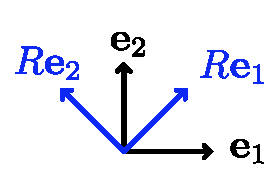
\includegraphics[width=.5\textwidth]{figures/OrientationPreserving.pdf}
    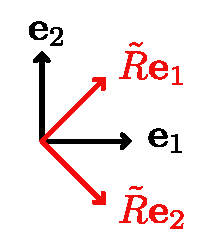
\includegraphics[width=.4\textwidth]{figures/OrientationNonPreserving.pdf}
    \captionsetup{font={scriptsize,sf}}
    \caption{Example of a orientation preserving (blue) and orientation non-preserving (red) transformation. The transformation that does not preserve orientation cannot be written in the usual form, \eqref{eq:2D:rotation:standard}.}
    \label{fig:orientation:non:preserving}
\end{marginfigure}
When you learn about the \emph{right-hand rule} in freshman physics or when the order of how one multiplies vectors matters---you are dealing with orientation. Orientation is the \emph{handedness} of a basis. 

Isometries that preserve the metric but change orientation are said to be \emph{disconnected from the identity}. This is in contrast to ordinary rotations $R(\theta)$ that are parameterize by some continuous parameter $\theta$ and satisfies $R(\theta = 0) = \one$. Instead, orientation changing isometries are the product of an orientation-preserving isometry with some \emph{discrete} symmetry, such as the matrix
\begin{align}
    \begin{pmatrix}
        1 & \pp 0 \\
        0 & -1
    \end{pmatrix}
\end{align}
in the example above. These discrete symmetries are called \emph{parities}. 

\begin{example}[Mirror universe] When you look into a mirror, you see a universe that looks identical to our own, except the image of yourself has changed their dominant hand. If you are right-handed, then your mirror image is left-handed. The reason for this is that the mirror universe is a parity transformation (reflection) of our own. If we draw an oriented basis in our universe with the $\ket{e_3}$ direction pointing into the mirror, then we observe the basis in the mirror universe $\ket{e'_i}$ to be the same except $\ket{e'_3} = -\ket{e_3}$. The isometry that takes vector components from our universe to the components in the mirror universe is
\begin{align}
    P = \begin{pmatrix}
        1 & & \\
        & 1 & \\
        & & -1
    \end{pmatrix} \ .
\end{align}
\end{example}

Isometries that are orientation changing, $\tilde R$, have determinant $-1$:
\begin{align}
\det \tilde R = -1 \ .     
\end{align}
The discrete symmetries (parities) that are at the heart of orientation-non-preserving isometries are significant in physics.  For example, the transformation that takes matter into antimatter is a combination of charge inversion and parity reflection. 

\begin{example}
Show that the product of an orientation-changing isometry (like parity) and an orientation-preserving isometry changes orientation. Show that the product of two orientation-changing isometries preserves orientation.
\end{example}

Tensors that change sign under a reflection are called \textbf{pseudo-tensors}\index{pseudo-tensors}. 
\begin{exercise}
Show that angular momentum is a pseudo-tensor. What other objects in classical mechanics and electrodynamics are pseudo-tensors?
\end{exercise}


\section{Determinant of a Product}
\label{sec:determinant:of:product}

We now prove the following handy relation for the determinant of a product of matrices:
\begin{align}
    \det MN = (\det M)(\det N) \ .
    \label{eq:det:product:rule}
\end{align}
As a corollary, this also tells us that
\begin{align}
    \det M\inv = (\det M)\inv \ .
\end{align}

Armed with our Levi-Civita definition of the determinant \eqref{eq:levi:civita:determinant:definition}, we may derive this rigorously.
\begin{exercise}
Even without a mathematically rigorous definition, argue that the multiplication rule above is true based on the interpretation of the determinant as the volume of a parallelpiped. 
\end{exercise}
% \begin{wide}
Starting from \eqref{eq:levi:civita:determinant:definition:totally:antisymmetrized}, we may invoke our antisymmetry gynmastics:
\begin{align}
    \det MN &= 
    \epsilon_{i_1 \cdots i_d}
    (MN)\aij{i_1}{1}\cdots (MN)\aij{i_d}{d} 
    \\
    &= 
    \epsilon_{i_1 \cdots i_d}
    M\aij{i_1}{j_1}N\aij{j_1}{1}
    \cdots 
    M\aij{i_d}{j_d}N\aij{j_d}{d}
    \\
    &= 
    \epsilon_{i_1 \cdots i_d}
    M\aij{i_1}{[j_1}
    \cdots 
    M\aij{i_d}{j_d]}
    N\aij{j_1}{1}
    \cdots
    N\aij{j_d}{d}
    \\
    &= 
    \epsilon_{i_1 \cdots i_d}
    M\aij{i_1}{[j_1}
    \cdots 
    M\aij{i_d}{j_d]}
    N\aij{[j_1}{1}
    \cdots
    N\aij{j_d]}{d}
    \\
    &= 
    \epsilon_{i_1 \cdots i_d}
    M\aij{i_1}{1}
    \cdots 
    M\aij{i_d}{d}\quad
    \epsilon_{j_1 \cdots j_d}
    N\aij{j_1}{1}
    \cdots
    N\aij{j_d}{d}
    \\
    &= 
    (\det M)
    (\det N)
    \ .
\end{align}
% \end{wide}
\begin{exercise}
Justify each step of the above derivation using the antisymmetry gymnastic techniques from Section~\ref{sec:antisymmetric:dynamics}.
\end{exercise}

\begin{exercise}
Prove $\det M\inv = (\det M)\inv$ for the specific case of a $2\times 2$ matrix. Use the facts that
\begin{align}
    \det 
    \begin{pmatrix}
        a & b \\
        c & d
    \end{pmatrix}
    &= 
    ad - bc
    &
    \text{and}&
    &
    \begin{pmatrix}
        a & b \\
        c & d
    \end{pmatrix}\inv 
    =
    \frac{1}{ad-bc}
    \begin{pmatrix}
        \pp d &   -b \\
          -c &  \pp a
    \end{pmatrix}
    \ .
\end{align}
\end{exercise}





% Does this make sense?

% then show that you get an inverse


% *******
% put in a discussion of diffeomorphisms when talking about transformations...
% in this class we talk about rotations, but most of the statements
% are true for more general transformations until we get to metric spaces
% at which point we care about preserving orhtonormal bases





% pseudotensor
% some identities, how to find them
% upper index
% where does it come from? idea that symmetric part and antisymmetric part decouple



\section{Cross Products and Levi-Civita}
\label{sec:cross:product}

In \eqref{eq:det:eps:v:w} you may have recognized that $\epsilon_{ijk}v^j w^k$ to be a familiar object: it is the $i^\text{th}$ component of the three-space cross product:\sidenote{This is sometimes written $\vec{v}\wedge\vec{w}$, which I first saw in the Landau \& Lifschitz textbooks. The wedge product has come to mean a generalized antisymmetric product in differential geometry and algebraic geometry.}
\begin{align}
    \vec{v}\times \vec{w} = 
    \begin{pmatrix}
        v^2w^3 - v^3w^2 \\
        v^3 w^1 - v^1w^3 \\
        v^1 w^2 - v^2 w^1
    \end{pmatrix}
    \ .
\end{align}
What we recognize is that $\epsilon_{ijk}v^j w^k$ has a \emph{lower} index. In a metric space we may raise this index to create an object that transforms like a vector under rotations
\begin{align}
    g^{i\ell}\epsilon_{\ell j k}v^j w^k \ .
\end{align}
This looks like a tensor, but it is in fact a pseudotensor.\sidenote{More accurately, it looks like a vector, but it is actually a pseudovector or axial vector.} Under a reflection, both $v$ and $k$ pick up signs, but so too does $\epsilon_{\ell j k}$. 

We see that the cross product is simply the Levi-Civita symbol pre-loaded with two vectors. The result is a dual pseudo-vector. This is a manifestation of the Hodge duality in \eqref{eq:Hodge:duality:epsilon}. In four dimensions, the analogous operation returns a totally antisymmetric (0,2) tensor:
\begin{align}
    \epsilon_{\mu\nu\rho\sigma}v^\rho w^\sigma \ .
\end{align}
This explains why the cross product is only defined in three dimensions. 


\section{Dependence on the Metric?}

You may think that there is a bit of a conceptual puzzle. The metric was what allowed us to define any notion of length. The Levi-Civita symbol is defined completely independently of the metric. The determinant of a matrix, $M$, in turn is defined with respect to the Levi-Civita symbol and is identified with the volume of a parallelpiped. In what way is the determinant able to define a volume if it does not seem to use the metric? 

Part of the answer here is that the determinant gives an \emph{oriented}\sidenote{We say oriented because the sign of the determinant is negative if the vectors $M\ket{e_i}$ differ by orientation compared to the basis $\ket{e_i}$. To see this, consider the matrix $M$ that simply flips the $\ket{e_1}$ and $\ket{e_2}$ vectors.} volume relative to the volume of the unit [hyper-]cube formed out of the basis vectors. Another way to see this is to appeal to Figure~\ref{fig:det:vis:boxes} where we may see that our identification of $\det M$ in two dimensions with an area invoked areas of boxes whose sides are length $M\aij{i}{j}$. These components of $M$, in turn, are a result the action of dual vectors acting on the $M\ket{e_j}$, \eqref{eq:det:v1:inner:prod}--\eqref{eq:det:w2:inner:prod}. These dual vectors are defined relative to the metric, and so it is here that some sense of measure enters: not in the definition of the determinant, but in the interpretation of that definition as a volume.

\begin{subappendices}
\section{Levi-Civita Identities}

You may find yourself contracting Levi-Civita symbols. The antisymmetry of the indices gives a hint for how to resolve these. Consider the contraction
\begin{align}
\epsilon_{ijk}\epsilon^{nmk}
= c \, \delta^{[n}_{[i}\delta^{m]}_{j]}    
\label{eg:product:of:Levi:Civita:example}
\end{align}
where we recall that the square brackets mean \emph{antisymmetrize and average over all the terms in the sum}, so that 
\begin{align}
    T^{[i_1\cdots i_n]} \defeq \frac{1}{n!}
    \left(  
        T^{12\cdots n}
        - T^{21\cdots n}
        + \cdots
    \right) \ .
\end{align}
In \eqref{eg:product:of:Levi:Civita:example} we have posited that the contraction on the left-hand side is some sum over Kronecker $\delta$s. We have then used the antisymmetry of the uncontracted indices on the left-hand side to impose antisymmetry onto those indices on the right-hand side. 

You should stop to think: \emph{why} do we know that the right-hand side is a sum of terms that are are products of Kronecker $\delta$s? The glib answer is: \emph{what else could it be?} We have no other invariant tensors lying around. You may wonder if we could use the metric $g_{ij}$ or its inverse $g^{ij}$. We cannot for two reasons, one ideological and one practical:
\begin{enumerate}
    \item Ideologically, the Levi-Civita tensor does not invoke the metric in its definition. This means that we could have defined it on a space \emph{without} a metric and so the contraction \eqref{eg:product:of:Levi:Civita:example} should not depend on the metric.
    \item Practically, the metric and its inverse are symmetric in its indices. On the right-hand side of \eqref{eg:product:of:Levi:Civita:example}, all the indices of the same height are antisymmetrized. This means that any terms that include the metric would identically vanish. 
\end{enumerate}
So this leaves us with the Kronecker $\delta$s. All that remains is to find the value of the coefficient $c$. In practice, the easiest way to do this is to simply pick any non-vanishing choice of uncontracted indices to solve for it:
\begin{align}
    \epsilon_{12k}\epsilon^{12k} &=
    \epsilon_{121}\epsilon^{121} 
    +
    \epsilon_{122}\epsilon^{122}
    +
    \epsilon_{123}\epsilon^{123}
    = 
    1 
    \\
    &= \frac{c}{(2!)^2}
    \left(
    \delta^1_1 \delta^2_2 
    - \delta^1_2 \delta^2_1
    -
    \delta^2_1 \delta^1_2 
    + \delta^2_2 \delta^1_1
    \right)
    =\frac{c}{2} \ ,
\end{align}
from which we derive $c=2$, and thus we find the identity
\begin{align}
\epsilon_{ijk}\epsilon^{nmk}
= 2 \, \delta^{[n}_{[i}\delta^{m]}_{j]}    \ .
\label{eg:product:of:Levi:Civita:example:answer} 
\end{align}
\begin{example}
Let us simplify the contraction $\epsilon_{ijk}\epsilon^{njk}$. We propose that this is simply proportional to the Kronecker $\delta$, since this is the only way to match the free indices:
\begin{align}
    \epsilon_{ijk}\epsilon^{njk} = c\, \delta^i_n \ . 
\end{align}
We match the coefficient $c$ by picking a non-zero value of the free indices:
\begin{align}
    \epsilon_{1jk}\epsilon^{1jk}
    &=
    \epsilon_{123}\epsilon^{123}
    +
    \epsilon_{132}\epsilon^{132}
    = 2 \ ,
\end{align}
where we do not bother writing terms where either $j$ or $k$ is 1 since those will be zero. This gives $c=2$. One can readily check that for $i\neq n$, $\epsilon_{ijk}\epsilon^{njk}\equiv 0$ because each term has at least one repeated index value. We thus derive 
\begin{align}
    \epsilon_{ijk}\epsilon^{njk} = 2\, \delta^i_n \ . 
\end{align}
\end{example}

In fact, we can do the general case.\sidenote{This is a good exercise. I am tempted to leave it as an exercise, but I want to write down the derivation before I forget how I solved it. You should attempt to solve it without looking at my solution. Even if you do not, you should justify each step that I make.} We start with the $d$ dimensional Levi-Civita symbol---this means that there are $d$ indices that each take values from 1 to $d$. Consider the contraction of $(d-p)$ indices between two Levi-Civita symbols:
\begin{align}
    \epsilon_{i_1\cdots i_p i_{p+1}\cdots i_d}\,
    \epsilon^{j_1\cdots j_p i_{p+1}\cdots i_d}
    &=
    c\, \delta^{[i_1}_{[j_1}\delta^{i_2}_{j_2} \cdots \delta^{i_p]}_{j_p]} \ .
    \label{eg:product:of:Levi:Civita:general}
\end{align}
Let us assume that the signature of the metric is $\sgn{g}=+1$, as it is in Euclidean space. First we assume that $i_1, \cdots, i_p$ and $j_1, \cdots, j_p$ are chosen such that it is possible to have non-zero terms. Consider the left-hand side. This is a sum of the form:
\begin{align}
    \epsilon_{i_1\cdots i_p i_{p+1}\cdots i_d}\,
    \epsilon^{j_1\cdots j_p i_{p+1}\cdots i_d}
    &= 
    \sum_\sigma 
    \epsilon_{i_1\cdots i_p \sigma_1\cdots \sigma_{(d-p)}}\,
    \epsilon^{j_1\cdots j_p \sigma_1\cdots \sigma_{(d-p)}}
     \ .
\end{align}
where the right-hand side sums over all permutations of the $(d-p)$ contracted indices.\sidenote{We assume that the $\sigma_i$ are permutations of index values that produce non-zero terms.} Then each term on the right-hand side contributes the same value, which is either $\pm 1$ depending on the choice of the free indices. There aer a total of $(d-p)!$ permutations so we may write
\begin{align}
    \epsilon_{i_1\cdots i_p i_{p+1}\cdots i_d}\,
    \epsilon^{j_1\cdots j_p i_{p+1}\cdots i_d}
    &= 
    (d-p)!\,
    \epsilon_{i_1\cdots i_p \hat\sigma_1\cdots \hat\sigma_{(d-p)}}\,
    \epsilon^{j_1\cdots j_p \hat\sigma_1\cdots \hat\sigma_{(d-p)}}
     \ ,
\end{align}
where there is \emph{no sum} over the $\hat\sigma_i$; it is understood that we are picking some reference choice of the contracted indices for which neither Levi-Civita symbol vanishes. We understand that the right-hand side is either $\pm (d-p)!$ depending on whether the choice of $\{i_n\}$ and $\{j_m\}$ are even of odd permutations of one another. 

Now tackle the right-hand side of \eqref{eg:product:of:Levi:Civita:general}. The antisymmetrized product of Kronecker $\delta$s is
\begin{align}
    \delta^{[i_1}_{[j_1}\delta^{i_2}_{j_2} \cdots \delta^{i_p]}_{j_p]}
    &=
    \frac{1}{(p!)^2}
    \left( 
    \delta^{i_1}_{j_1}\delta^{i_2}_{j_2} \cdots \delta^{i_p}_{j_p}
    + \cdots
    \right) \ .
\end{align}
The omitted terms are all antisymmetric permutations of indices of the same height. There are a total of $(p!)^2$ such terms.  For a given choice of indices $\{i_n\}$ and $\{j_m\}$ how many of these terms are non-zero? A term is only non-zero if the ordered list of upper indices \emph{exactly} matches the ordered list of lower indices. For a given permutation of the $\{i_n\}$ indices, there is exactly one choice of the $\{j_n\}$ indices that matches it. Since there are $p!$ such permutations of the $\{i_n\}$ indices, there is a total of $p!$ non-zero terms. Further more, each of these terms has the same sign: to go from any one non-zero term to any other non-zero term, you do the same number of permutations of the upper indices and lower indices. Thus you get the same number of sign flips in the $[\cdots]$ antisymmetrization of the indices. As a result, the right-hand side of \eqref{eg:product:of:Levi:Civita:general} is
\begin{align}
    c\,
    \delta^{i_1}_{[j_1}\delta^{i_2}_{j_2} \cdots \delta^{i_p}_{j_p]} \ .
\end{align}
We understand that this is equal to $\pm c/p!$ because exactly one term is non-zero in the antisymmetrized sum of terms. Note that the $\pm$ here matches the same $\pm$ on the left-hand side.

All that remains is to match the two sides to each other to determine the value of $c$. The simplest choice is to set $i_n = j_n = n$ for $1\leq n \leq p$. This gives
\begin{align}
    (d-p)!
    \epsilon_{1\cdots p (p+1)\cdots d}\,
    \epsilon^{1\cdots p (p+1)\cdots d}
    =
    \frac{c}{p!}
    \delta^{1}_{1}\delta^{2}_{2} \cdots \delta^{p}_{p} \ .
\end{align}
On the left-hand side we have chosen a convenient reference permutation to be $\hat \sigma_n = n$ for $p < n \leq d$. The Levi-Civita and Kronecker factors evaluate to one and we are left with $c= p! (d-p)!$. 




Overall sign depending on the sign of the metric. 


\section{The Levi-Civita Tensor versus Symbol}
\label{sec:Levi:Civita:Tensor:vs:Symbol}

The Levi-Civita symbol $\epsilon_{i\cdots k}$ is \emph{not} formally a tensor.\sidenote{This section is not part of the main narrative of this course, though the material is helpful for future study. It may be skipped on a first reading.} Maybe I should not even tell you that---in a standard linear algebra course, the observation that the Levi-Civita symbol is not a tensor is so far afield that it is usually one of those little lies that we permit because they are eventually rectified in the special cases where they need to be. However, the cases where it matters that the Levi-Civita symbol is \emph{not} tensorial are often those that show up in physics! As such, I owe it to you to explain why physicists say the Levi-Civita symbol is not a tensor, and why we go out of our way to define a bona fide Levi-Civita tensor.\sidenote{For a more in-depth discussion, I encourage you to pick up your favorite textbook on general relativity. I recommend Sean Carroll's \emph{Introduction to Spacetime and Geometry}. If you have made it this far into this course, all you need is a little bit of familiarity with vector calculus to begin learning the differential geometry that girds relativity.}

\subsection{Why you should be skeptical} 

Just because $\epsilon_{i\cdots k}$ has indicies that does \emph{not} mean that it is a tensor! This \emph{symbol} is defined \emph{by fiat} by \eqref{eq:def:levi:civita:d:dim:upper} and by \eqref{eq:Levi:Civita:symbol:definition:d:dim} for its upper-indexed cousin. This definition set for \emph{any} basis. In contrast, when you specify the components of a matrix, it is understood that those components are with respect to some basis. If you go to a different basis, then the components of the matrix change. The fact that $\epsilon_{i\cdots k}$ does \emph{not} change should make you suspect that it is not an honest tensor.
\begin{example}
The only tensor whose components are defined \emph{by fiat} that is \emph{actually} a tensor is the Kronecker $\delta$. Under a rotation, $\delta^i_j \to R\aij{i}{k}(R\inv)\aij{k}{j} = \delta^i_j$.
\end{example}

Let us diagnose this. If we \emph{pretend} that $\epsilon_{i\cdots k}$ \emph{is} an honest tensor, then it would transform according to our tensor transformation rule \eqref{eq:transformation:of:upper:and:lower:indices}:
\begin{align}
    \epsilon_{i_1\cdots i_d} \to 
    (R\inv)\aij{j_1}{i_1}\cdots
    (R\inv)\aij{j_d}{i_d}
    \epsilon_{j_1 \cdots j_d} 
    =
    (\det R)\inv \epsilon_{i_1\cdots i_d}
    \label{eq:transformation:of:Levi:Civita:symbol:if:it:were:a:tensor}
    \ .
\end{align}
\begin{exercise}
Prove \eqref{eq:transformation:of:Levi:Civita:symbol:if:it:were:a:tensor} assuming that $\epsilon_{i_1\cdots i_d}$ transforms like a tensor.
\end{exercise}
As long as we consider orientation preserving isometries $R$, $\det R =1$ and the $\epsilon_{i \cdots k}$ symbol's definition\sidenote{The definition is that the Levi-Civita tensor is the same in any basis.} is consistent with its transformation as an honest tensor. However, if the transformation $R$ is orientation non-preserving, then the Levi-Civita symbol picks up a sign and we are reminded that this is not quite a proper tensor. The appearance of this sign is why the Levi-Civita symbol is sometimes called a \textbf{pseudo-tensor}.

% \paragraph{Is the upper-index Levi-Civita tensor defined consistently?}
\subsection{Consistent Upper-Index Levi-Civita}
In \eqref{eq:def:levi:civita:d:dim:upper} we have cavalierly \emph{defined by fiat} an upper-indexed version of an existing tensor. Alarm bells should be ringing! If we are in a metric space, then this object is \emph{already defined} with respect to the inverse metric:
\begin{align}
    \epsilon^{i_1\cdots i_d}
    \equiv
    g^{i_1j_1}
    \cdots
    g^{i_dj_d}
    \epsilon_{j_1\cdots j_d}
    \stackrel{?}{=}
    (\det g^{\cdot\cdot}) \;
    \epsilon^{i_1\cdots i_d} \ .
    \label{eq:det:raised:index:det:g}
     \ .
\end{align}
In the last step we recognize the definition of the determinant of $g^{ij}$. This expression appears to only make sense if $\det g = 1$.\sidenote{Sometimes this factor of $\det g^{\cdot\cdot}$ is built into the definition of the upper-indexed Levi-Civita tensor.}
\begin{exercise}
Prove the last equality of \eqref{eq:det:raised:index:det:g}. The point here is to show that the antisymmetry in the $j_n$ indices induces an antisymmetry in the $i_n$ indices. \textsc{Hint}: as with many problems, it helps to write out a low-dimensional example explicitly.
\end{exercise}

When is $\det g = 1?$ This condition is certainly true for the Euclidean metric in the standard basis. 
\begin{exercise}
Show that $\det g =1$ in Minkowski space with an odd number of spacetime dimensions, but $\det g = -1$ in Minkowski space with an even number of spacetime dimensions. We assume that there is only one timelike direction. In four spacetime dimensions the upper-index Levi-Civita symbol is not a tensor due to this minus sign.
\end{exercise}
In fact, it seems that we are asking the wrong question. The metric defines the length of vectors. If the determinant is positive but not one, then it may simply be a matter of defining properly normalized basis vectors. We thus see that if we are in an orthonormal basis, the upper-index Levi-Civita symbol---whose components are defined by fiat---is \emph{almost} consistent with its definition with respect to the inverse metric raising the indices of the lower-index Levi-Civita symbol. The \emph{almost} boils down to a sign coming from the determinant of the metric.

In fact, there is a simple solution to this. The sign of the determinant of the metric, $\sgn g$, is simply a property of your spacetime.\sidenote{We say `spacetime' because the typical places where you have $\sgn g = -1$ is coming from the relative sign between space and time.} Below \eqref{eq:def:levi:civita:d:dim:upper} we observed that the overall sign in front of the upper-index Levi-Civita symbol $\epsilon^{i\cdots k}$ is a choice. We see that we can get rid of the issue of the sign of $\det g^{\cdot\cdot}$ by simply redefining \eqref{eq:def:levi:civita:d:dim:upper} to be:
\begin{align}
    \epsilon^{i_1\cdots i_d}
    \defeq
    \sgn g\; 
    \epsilon_{i_1\cdots i_d} \ .
    \label{eq:def:levi:civita:d:dim:upper:with:sign}
\end{align}
All we are doing here is \emph{choosing} a convention for the definition of upper-indexed Levi-Civita symbol.

\subsection{Problems on a Bundle} 

Thus far we have quibbled over factors of a sign coming from either the determinant of the isometry or the determinant of the metric. If we happen to be in a space where our basis is such that $\det g = 1$ and if we restrict ourselves to only isometries with $\det R = 1$, then we could be forgiven for treating the Levi-Civita symbols as tensors. But it turns out that the situation is actually a bit more dismal.

 
In a metric space, we could simply rescale an orthogonal basis to satisfy $\det g =1$. However, when we have not just \emph{one} metric space, but a \emph{bundle} of metric spaces over a manifold---in the sense of Chapter~\ref{ch:bundles}---then it is not always the case that $\det g =1$ for \emph{every} tangent space on the bundle.\sidenote{This is the scenario in general relativity, but also in more the prosaic case of polar coordinates in Section~\ref{sec:polar:coordinates}. }
% 

In the bundle picture, the metric is a function of the base spacetime, $g(x)_{ij}$. 
% 
% 
We want our would-be-tensors to transform \emph{tensorially} with respect to change of coordinates $x \to  y(x)$. This is called \textbf{diffeomorphism invariance}\index{diffeomorphism invariance}.  In Chapter~\ref{ch:bundles} we saw that partial derivatives are the natural basis vectors on the tangent bundle. In this sense, the transformations at each tangent plane are
\begin{align}
    R\aij{a}{i} = \frac{\partial y^a}{\partial x^i}
\end{align}
under which vectors transform as
\begin{align}
    \frac{\partial}{\partial x^i} \to 
    \frac{\partial y^a}{\partial x^i} \frac{\partial}{\partial y^a}
    = R\aij{a}{i} \, \frac{\partial}{\partial y^a} \ .
\end{align}
It is with respect to the `rotation' matrices $R\aij{a}{i}$ that we would like all our objects to transform according to tensors. 
% 
This means that the metric $g(x)_{ij}$, which is a function of the base spacetime, transforms as
\begin{align}
    g(y)_{ab} = \frac{\partial x^i}{\partial y^b}  \frac{\partial x^j}{\partial y^b} g(x)_{ij}
    = (R\inv)\aij{i}{a} (R\inv)\aij{j}{b} g(x)_{ij} \ .
\end{align}
We used $R\inv = (\partial x/\partial y)$. Take the determinant of both sides gives\sidenote{The determinant of the metric is an index-free quantity that transforms. This cannot be a tensor. Instead, it is called a \emph{tensor density}. This is because $\det R$ scales like a volume. Because $\det g_{\cdot\cdot}$ transforms as $(\det R)^{-2}$, we say that it transforms as a tensor density with \emph{weight} $-2$. (The definition of the sign of the weight is up to convention.)}
\begin{align}
    \det g(y)_{\cdot\cdot} = (\det R)^{-2} \det g(x)_{\cdot\cdot} \ ,
    \label{eq:transformation:of:det:g}
\end{align}
where we simply invoke the rule for the determinant of a product of matrices \eqref{eq:det:product:rule}. We write $\det g_{\cdot\cdot}$ to indicate that we are taking the determinant of the metric rather than the inverse metric.\sidenote{Most other references simply write $\det g$ or, even more succinctly, $g$. In those references it is understood that $g$ is ``the one with the lower indices.'' We err on the side of pedagogical clarity.} We find that under diffeomorphisms:
\begin{enumerate}
    \item The both the lower-indexed and upper-indexed Levi-Civita symbol is not invariant because in general $\det R \neq 1$.
    \item The upper-index Levi-Civita symbol is not consistently defined relative to the lower-indexed symbol\sidenote{and vice versa.} because $\det g \neq 1$. In fact, $\det g$ itself transforms with diffeomorphisms.
\end{enumerate}
And so here we are. In the bundle construction of tangent spaces on a spacetime manifold, the diffeomorphism invariance of the manifold induces transformations on the tangent spaces. We want to treat these transformations as isometries on each tangent space. This means that under a change of coordinates $x^i \to y(x)^a$, objects with respectively upper and lower indices transform as
\begin{align}
    v(x)^i &\to v(y)^a = \frac{\partial y^a}{\partial x^i} v(x)^i
    = R\aij{a}{i}v(x)^i
    \\
    w(x)_i &\to w(y)_a = \frac{\partial x^i}{\partial y^a} w(x)_i 
    = (R\inv)\aij{i}{a}w_i 
    \ .
\end{align}
The objects $v(x)^i$ and $w(x)_i$ are \textbf{vector fields}\index{vector field}---or more generally, tensor fields\index{tensor field}. They generalize the notion of a tensor in a single vector space: at each position $x$, $v(x)^i$ is a vector in the vector space that is the tangent plane at $x$. The problem is that we would like to be able to use the Levi-Civita symbol on these tangent planes. But now the issues above rear their heads: because $\det R \neq 1$ and $\det g_{\cdot\cdot} \neq 1$, the Levi-Civita symbol only takes the prescribed form in a specific basis. 

\subsection{Toward a Levi-Civita Tensor}

What we would like is to have is a version of the Levi-Civita symbol with the following properties:
\begin{enumerate}
    \item It must transform as a true tensor, \eqref{eq:transformation:of:Levi:Civita:symbol:if:it:were:a:tensor}.
    \item The definition must be invariant.
\end{enumerate}
We call this object the \textbf{Levi-Civita tensor} $\varepsilon_{i_1\cdots i_d}$. 
% 
In \emph{this} course the distinction is \emph{so} miniscule that the two symbols are \emph{almost} typographically identical.\sidenote{Other books may write $\bar\epsilon$ or $\tilde\epsilon$ for the Levi-Civita symbol.} How should we define $\varepsilon_{i_1\cdots i_d}$?

A diffeomorphism $x^i \to y(x)^a$ induces a tangent space transformation
\begin{align}
R\aij{a}{i} = \frac{\partial y^a}{\partial x^i}     \ .
\end{align}
A \textbf{tensor density}\index{tensor density} of \textbf{weight}\index{weight} $w$ is a quantity $t\aij{i\cdots j}{k\cdots \ell}$ that transforms like a tensor with an additional rescaling by $(\det R)^w$:
\begin{align}
    t\aij{i\cdots j}{k\cdots \ell} \to 
    \left(\det \frac{\partial y}{\partial x}\right)^w
    t\aij{a\cdots b}{c\dots d}
    \;
    \frac{\partial y^i}{\partial x^a}
    \cdots
    \frac{\partial y^j}{\partial x^b}\;
    \frac{\partial y^c}{\partial x^k}
    \cdots
    \frac{\partial y^d}{\partial x^\ell} \ .
\end{align}\sidenotetext{The determinant of the metric is so significant in geometric contexts that it is sometimes shortened as $g=\det g$.}
\begin{example}
We see that \eqref{eq:transformation:of:det:g} tells us that the determinant of the metric,\sidenotemark{} $\det g_{\cdot\cdot}$, is an index-free tensor density of weight $w=-2$:
\begin{align}
    \det g_{\cdot\cdot} \to \left(\det \frac{\partial x}{\partial y}\right)^2\, \det g_{\cdot\cdot}
    \label{eq:det:g:tensor:density}
    \ .
\end{align}
\end{example}

The Levi-Civita symbol is a tensor density.\sidenote{This is surprising! The Levi-Civita \emph{symbol} has no business to be a tensor density: it is defined to be the same in any basis. It was defined to have constant components rather than components that transform.} We can see how by starting with the definition of the determinant of a matrix, $M$:
\begin{align}
    \det M &=\epsilon_{i\cdots k} M\aij{i}{1}\cdots M\aij{k}{d}
    \\
    & =\epsilon_{i\cdots k} M\aij{i}{[1}\cdots M\aij{k}{d]}
    % \\
    % & =\epsilon_{i\cdots k} M\aij{i}{[a}\cdots M\aij{k}{c]} \epsilon^{a\cdots c} \
\end{align}
Now we may follow Example~\ref{eg:pull:out:epsilon}. The right hand side represents one component $T_{1\cdots d}$ of a totally antisymmetric tensor
\begin{align}
    T_{j\cdots \ell}
    \defeq
    \epsilon_{i\cdots k} M\aij{i}{[j}\cdots M\aij{k}{\ell]} \ .
\end{align}
The determinant definition gives $\det M = T_{1\cdots d}$. We then recover the totally antisymmetric tensor $T_{j\cdots \ell} = (\det M) \epsilon_{j\cdots \ell}$. This tells us that 
\begin{align}
    \epsilon_{j\cdots \ell} = (\det M)\inv 
    \epsilon_{i\cdots k} M\aij{i}{[j}\cdots M\aij{k}{\ell]} \ .
    \label{eq:epsilon:almost:transformation}
\end{align}
We may choose the matrix such that
\begin{align}
    M\aij{i}{j} = \frac{\partial x^i}{\partial y^j} \ .
\end{align}
we do this because then \eqref{eq:epsilon:almost:transformation} takes the form of the transformation of a tensor density of weight $w=-1$,
\begin{align}
    \epsilon_{j\cdots \ell} &= 
    \left(\det \frac{\partial x}{\partial y}\right)\inv 
    \epsilon_{i\cdots k} \frac{\partial x^i}{\partial y^j} \cdots \frac{\partial x^k}{\partial y^\ell} 
    \\
    &= \left(\det \frac{\partial y}{\partial x}\right)\phantom{\inv}
    \epsilon_{i\cdots k} \frac{\partial x^i}{\partial y^j} \cdots \frac{\partial x^k}{\partial y^\ell} 
    \ .
    \label{eq:epsilon:almost:transformation:dx:dy}
\end{align}
We see the Levi-Civita symbol \emph{appears} to transform as a tensor density of weight $w=+1$.\sidenote{Of course, $\epsilon_{i\cdots \ell}$ is defined to \emph{not} transform. Here we simply mean that this definition is consistent with the Levi-Civita symbol being a tensor density.} This means that if we want to define an honest Levi-Civita \emph{tensor} with the properties above, then we should multiply the Levi-Civita \emph{symbol} by some tensor density of weight $w=-1$ to cancel out the $\det \partial y/\partial x$ factor in \eqref{eq:epsilon:almost:transformation}.

The determinant of the metric \eqref{eq:det:g:tensor:density} gives us a natural object to do this. Since the determinant of the metric has weight $w=-2$, we know that $\sqrt{\det g_{\cdot\cdot}}$ has weight $w=-1$ as needed. We thus define the lower-indexed \textbf{Levi-Civita tensor}\index{Levi-Civita tensor} $\varepsilon_{i\cdots k}$ with respect to the Levi-Civita symbol $\epsilon_{i\cdots k}$ to be
\begin{align}
    \varepsilon_{i\cdots k} \defeq \sqrt{|\det g_{\cdot\cdot}|} \epsilon_{i\cdots k} \ .
    \label{eq:Levi:Civita:tensor:definition}
\end{align}
This is an tensor in the sense that when you apply a rotation `for each index' according to the tensor transformation laws, the resulting factors simplify to a determinant that cancels with the tensor density transformation of the $\sqrt{|\det g_{\cdot\cdot}|} $ factor. This means that $\varepsilon_{i\cdots k}$ is the same in any basis.
Observe that we have inserted an absolute value over the determinant of the metric. This is because we want this to make sense on a real vector space so all components should be real. There is nothing `deep' about this. In Euclidean space, $\det g_{\cdot\cdot} > 0$ so you can ignore the absolute value. In four-dimensional Minkowski space, $\det g_{\cdot\cdot} < 0$, so that you sometimes see $|\det g_{\cdot\cdot}|$ written as $(-\det g_{\cdot\cdot})$. The sign, however, does cause some headaches that you should keep track of carefully.


What about the upper-indexed tensor? Once we have defined $\varepsilon_{i\cdots k}$ in \eqref{eq:Levi:Civita:tensor:definition}, the upper-indexed object $\varepsilon^{i\cdots k}$ is uniquely specified by
\begin{align}
    \varepsilon^{i\cdots k}
    =
    g^{ia}\cdots g^{kc}
    \varepsilon_{a\cdots c} \ .
    \label{eq:Levi:Civita:tensor:definition:upper:gs}
\end{align}
% We want this to match the \emph{definition by fiat} in every basis,
% \begin{align}
%     \varepsilon^{i\cdots k} \stackrel{?}{\defeq} \sqrt{|\det g_{\cdot\cdot}|} \epsilon^{i\cdots k} \ .
%     \label{eq:Levi:Civita:tensor:definition:upper:fiat:maybe}
% \end{align}
The right-hand side of \eqref{eq:Levi:Civita:tensor:definition:upper:gs} is
\begin{align}
    g^{ia}\cdots g^{kc}
    \varepsilon_{a\cdots c}
    &=
    \sqrt{|\det g_{\cdot\cdot}|}
    \det{g^{\cdot\cdot}}
    \bar{\epsilon}^{i\cdots k}
    % \\&
    =
    \frac{\sgn{g}}{\sqrt{|\det{g_{\cdot\cdot}}|}}
    \bar{\epsilon}^{i\cdots k} 
    % \\
    % &= 
    % \frac{1}{\det{g_{\cdot\cdot}}} \varepsilon^{i\cdots k} 
    \ .
    \label{eq:raising:Levi:Civita:tensor:int}
\end{align}
We have used the fact that $g^{\cdot\cdot}$ is the inverse of $g_{\cdot\cdot}$ so that $\det{g^{\cdot\cdot}} = (\det g_{\cdot\cdot})\inv$.\sidenote{This was the reason why we put in the two dots in our notation for $\det g_{\cdot\cdot}$.} 
% 
We define\sidenote{This definition of $\bar\epsilon^{\cdots}$ is cumbersome. It is helpful to use it to clarify a choice for the overall sign of the upper-index Levi-Civita symbol. One common source of sign errors is to conveniently define $\epsilon^{1\cdots d}$ to match $\epsilon_{1\cdots d}$ in Euclidean space and then to carry that assumption into Minkowski space where one has to be careful about factors of $\sgn g$ that were not there in the Euclidean case.} $\bar\epsilon^{i\cdots k}$ to be the totally antisymmetric Levi-Civita symbol with upper indices and sign convention in \eqref{eq:def:levi:civita:d:dim:upper}, that is $\bar\epsilon^{1\cdots d} \defeq +\epsilon_{1\cdots d}$.
\begin{exercise}
Fill in the details of each equality in \eqref{eq:raising:Levi:Civita:tensor:int}. Use antisymmetry gymnastics to explain how the $\bar\epsilon^{i\cdots k}$ appears and why we specify a particular sign convention for it.
\end{exercise}
% 
In \eqref{eq:raising:Levi:Civita:tensor:int} factor of $\sgn g$, the sign of the metric determinant,\sidenote{Because the $\sgn g_{\cdot\cdot} = \sgn{g^{\cdot\cdot}}$ we do not need the little dots here.} is a bit curious, but it is simply there so that we could write $\det g_{\cdot\cdot} = \sgn{g}\; |\det g_{\cdot\cdot}|$, which in turn makes it easier to deal with square roots of this determinant. We have shown that the rule for using the inverse metric to raise indices tells us that
\begin{align}
    \varepsilon^{i\cdots k} = \frac{1}{\det{g_{\cdot\cdot}}} \varepsilon^{i\cdots k}  \ .
\end{align}

Is this sensible with our stated goals of defining a Levi-Civita tensor that is both an honest tensor and uniquely defined? Indeed it does. 
% 
The overall factor of $\sgn g$ may seem odd, but this is an overall sign that is simply a property of your metric space. In fact, just below \eqref{eq:def:levi:civita:d:dim:upper} we observed that the \emph{by fiat definition} of the upper-index Levi-Civita symbol includes an arbitrary choice of sign. In 
\eqref{eq:def:levi:civita:d:dim:upper:with:sign} we then showed that a convenient choice is to absorb $\sgn g$ sign into the definition of the upper-index Levi-Civita symbol:
\begin{align}
    \epsilon^{i_1\cdots i_d}
    \defeq
    (\sgn g) \;
    \epsilon_{i_1\cdots i_d} \ .
\end{align}
With this understanding, \eqref{eq:raising:Levi:Civita:tensor:int} becomes
\begin{align}
    \varepsilon^{i\cdots k}
    = \frac{\epsilon^{i\cdots k}}{\sqrt{|\det g_{\cdot\cdot}|}}  \ .
\end{align}

\begin{exercise}
Show that the upper-index Levi-Civita tensor transforms as a tensor under diffeomorphisms. Compare and contrast this proof to the case of the lower-index Levi-Civita tensor. The proof is completely analogous, except you should be clear where factors of $\partial y/\partial x$ are replaced by factors of $\partial x/\partial y$ and vice versa.
\end{exercise}

\begin{exercise}
Show that the upper-index Levi-Civita tensor is an inverse of the lower-index tensor in the sense that
\begin{align}
    \varepsilon^{i\cdots k}\varepsilon_{i\cdots k} = n! \ .
\end{align}
% I should check this for signs
\end{exercise}

\end{subappendices}
